\chapter{Introducción específica} % Main chapter title

El presente capítulo describe los elementos componentes del sistema, el principio de funcionamiento y los requerimientos acordados con el cliente sobre el sistema.


\label{Chapter2}

%----------------------------------------------------------------------------------------
%	SECTION 1
%----------------------------------------------------------------------------------------


\section{Elementos componentes del sistema}
\label{sec:elementos_componentes_sistema}

Para entender el funcionamiento del sistema, es necesario conocer los elementos que lo componen. La presente sección describirá tanto los elementos físicos necesarios para conocer al sistema que se busca representar, como las herramientas de software utilizadas para el desarrollo del emulador.

\subsection{Elementos físicos del sistema}
\label{subsec:elementos_fisicos}

La presente sección dará una descripción general de los elementos que serán de vital importancia para el proyecto.

\subsubsection{Bootloader}
\label{subsec:bootloader}

El \textit{bootloader} es una pieza de software relativamente simple, cuyo principal objetivo es cargar el software de vuelo en la memoria RAM del sistema. Una vez cargado el software de vuelo, le cede el control al software de vuelo, el cual se encarga de ejecutar la misión del sistema.

En misiones espaciales es común que el \textit{bootloader} tenga la capacidad de verificar la integridad del software de vuelo antes de cargarlo en la memoria RAM, así mismo, de cargar diferentes versiones del software de vuelo en caso de que alguna de ellas se encuentre dañada.

\subsubsection{Firmware}
\label{subsec:firmware}

El \textit{firmware} es un software que se encuentra almacenado en la memoria no volátil del sistema, y es el encargado de inicializar los periféricos del sistema. Usualmente, este componente es desarrollado por un equipo especializado tanto en la misión para la que se está desarrollando el sistema, como en la arquitectura del microprocesador que se está utilizando. En el caso de aplicaciones espaciales, el \textit{firmware} es llamado software de vuelo o \textit{Fly Software} (FSW).

Normalmente, en la memoria no volátil del sistema se almacenan múltiples versiones del software de vuelo. Varias de ellas están presentes para servir de redundancia, en caso de que alguna de ellas se encuentre dañada, como para almacenar distintas versiones del software de vuelo con modos de operación más limitados pero seguros.

\subsubsection{Unidad de procesamiento}
\label{subsec:unidad_procesamiento}
Todo lo previamente mencionado se ejecuta en la unidad de procesamiento o CPU. La CPU es el componente encargado de ejecutar las instrucciones tanto del \textit{bootloader} como del software de vuelo.

El CPU interactúa con los periféricos del sistema, especialmente con la memoria RAM del sistema, ya que es el medio de almacenamiento masivo de alta velocidad de acceso.

El CPU, una vez encendido, empezará a leer las instrucciones de una posición dada por el fabricante y ejecutarlas secuencialmente. Es deber del desarrollador posicionar al \textit{bootloader} en esa posición de memoria.

\subsection{Software utilizado}
\label{subsec:software_utilizado}

La presente sección describirá las herramientas de software que fueron utilizadas para el desarrollo del trabajo.

\subsubsection{C++}
\label{subsec:cpp}

Dado que el emulador es un software que simula el comportamiento de un CPU, es necesario que el lenguaje de programación utilizado sea de bajo nivel, permitiendo mejores tiempos de ejecución y un mayor control sobre los recursos utilizados. Por lo tanto, se decidió utilizar C++ como lenguaje de programación para el desarrollo del emulador.

Otro motivo para su elección es que C++ es un lenguaje de programación ampliamente utilizado en la industria, por lo que facilita la comunicación con otros desarrolladores y la integración con otros sistemas.

\subsubsection{Herramientas Clang}
\label{subsec:clang_tidy}

Se utilizó Clang Tidy como herramienta de análisis estático de código. Permitiendo una mayor calidad del código y sintaxis uniforme. Así mismo se forzaron reglas para evitar malas prácticas comunes en los lenguajes de programación de bajo nivel, tales como el uso de memoria no inicializada, o aritmética de punteros.

También se utilizó Clang Format para mantener un estilo de código uniforme en todo el proyecto.

\subsubsection{Latex}
\label{subsec:latex}

Se utilizó Latex como herramienta de escritura de la documentación para el manual de usuario del proyecto. Dicha elección se tomo debido a que Latex es una herramienta ampliamente utilizada en la industria para la escritura de documentos técnicos.

El manual de usuario busca ser una guía completa y en detalle de la herramienta, no solo explicando la interfaz expuesta, sino decisiones de diseño y funcionamiento interno de la herramienta.

\subsubsection{Doxygen}
\label{subsec:doxygen}

Se utilizó Doxygen como herramienta de generación de documentación del código fuente. Con esta herramienta se generó un sitio web el cual describe la interfaz para interactuar con la herramienta (API). Dicha documentación busca ser una guía rápida para desarrolladores que estén utilizando el emulador.


\section{Principio de funcionamiento}
\label{sec:principio_funcionamiento}

El funcionamiento de un CPU, y por lo tanto de un emulador, se puede mostrar de manera simplificada de forma gráfica:

\begin{figure}[htbp]
	\centering
	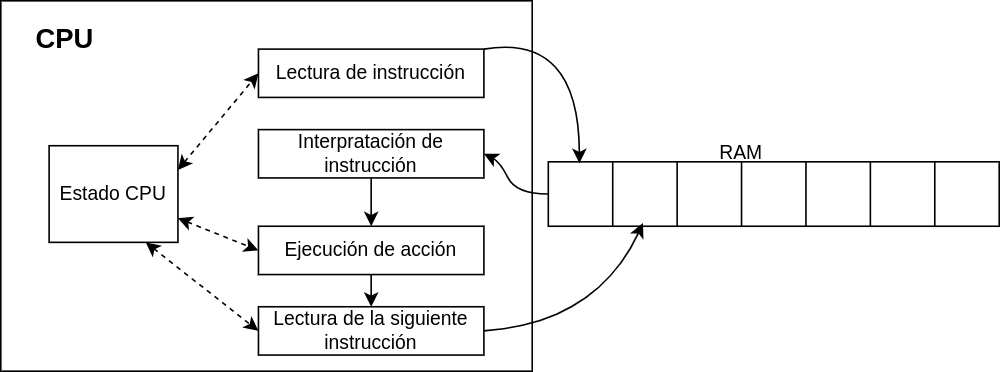
\includegraphics[width=1\textwidth]{./Figures/funcionamiento_emulador}
	\caption{Funcionamiento de alto nivel de un CPU o emulador.}
	\label{fig:functionamiento_emulador}
\end{figure}

Dicho flujo se ejecuta de manera continua, y no necesariamente las instrucciones se ejecutan en el orden en el que se encuentran en la memoria. Esto se debe a que el CPU tiene instrucciones de salto condicional, instrucciones de salto incondicional, y puede recibir interrupciones que cambien el flujo de ejecución del programa.


Un desafío que se tuvo que resolver temprana en el desarrollo del emulador fue la endianess del sistema. El endianess es el orden en el que se almacenan los bytes en la memoria. En el caso de la arquitectura SPARC V8, se utiliza el ordenamiento \textit{big-endian}, lo que significa que el byte más significativo se almacena en la dirección de memoria más alta. Por otro lado, la arquitectura x86 (Es decir, nuestros computadoras de escritorio) utiliza el ordenamiento \textit{little-endian}, donde el byte menos significativo se almacena en la dirección de memoria más baja. Por lo tanto, al momento de interpretar los datos obtenidos de la memoria, se debe reordenar los bytes para que tengan sentido. Dicha problemática es propia únicamente del emulado

\section{Requerimientos}
\label{sec:requerimientos}

